\documentclass{beamer}
\mode<presentation>{
  \usetheme{Warsaw}

  \definecolor{beamer@blendedred}{rgb}{0.7,0.1,0.1}
  \setbeamercolor{structure}{fg=beamer@blendedred}

  \setbeamercovered{invisible}
}

\usepackage[T2A]{fontenc}
\usepackage[utf8]{inputenc}
\usepackage[russian]{babel}
\usepackage{multimedia}
\logo{
\includegraphics[height=0.3cm]{valknut.png}}



\title{Зачем ФП?}
\author{Максим Трескин\\ \texttt{maxim.treskin@gmail.com} \\ \texttt{@mtreskin}}
\date[2010.10.02]{2 октября, 2010}

\begin{document}

\begin{frame}
  \titlepage
\end{frame}




\begin{frame}
  \frametitle{Функциональное программирование}
  \begin{itemize}
  \item Сначала был матан: Алонзо Чёрч придумал $\lambda$-исчисления
    \pause
  \item Затем практика: Джон Маккарти открыл Lisp, содержащий реализацию $\lambda$-исчисления
  \end{itemize}
\end{frame}


\begin{frame}
  \frametitle{В чём соль?}
  \begin{itemize}
  \item Не изменяется состояние
    \pause
  \item Хвостовая рекурсия
    \pause
  \item Функции первого класса
    \pause
  \item Алгебраические типы и сопоставление шаблону
  \end{itemize}
\end{frame}

\begin{frame}
  \frametitle{Неизменяемое состояние}
  \begin{itemize}
  \item Сложно накосячить
    \pause
  \item Легко тестировать
    \pause
  \item Легко распределять
  \end{itemize}
\end{frame}


\begin{frame}[fragile]
  \frametitle{Хвостовая рекурсия}
  \begin{block}{}
\begin{verbatim}
State = {inc:integer = 0}

iterate(State) ->
    NewState = State{inc + 5}
    iterate(NewState)
\end{verbatim}
  \end{block}

\end{frame}


\begin{frame}
  \frametitle{Обычное выполнение рекурсии}
  \begin{itemize}
  \item Записали на стек адрес, куда надо вернуться
    \pause
  \item Вызвали функцию с начальными параметрами
    \pause
  \item Записали на стек адрес, куда надо вернуться
    \pause
  \item Вызвали функцию с новыми параметрами
    \pause
  \item Повторить до завершения памяти
  \end{itemize}
\end{frame}

\begin{frame}
  \frametitle{Xzibit, прокачай нашу рекурсию}
  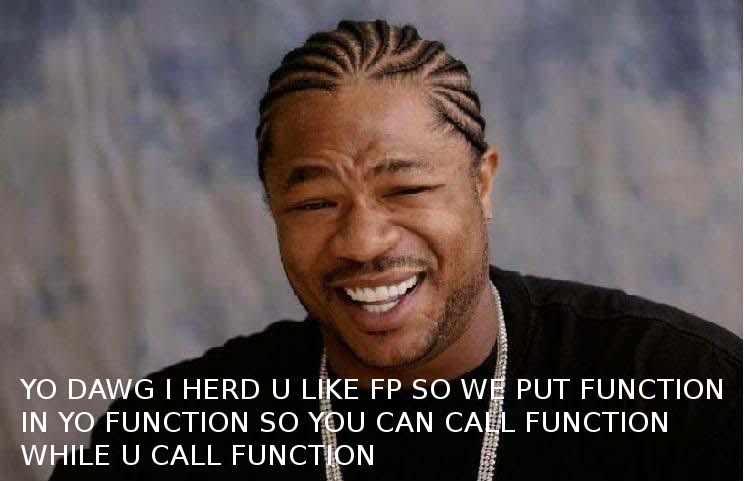
\includegraphics{xzibit-happy.png}
\end{frame}

\begin{frame}
  \frametitle{Xzibited выполнение рекурсии}
  Транслятор преобразует хвостовую рекурсию в итерацию!
  \pause
  \begin{itemize}
  \item Записали на стек адрес, куда надо вернуться
    \pause
  \item Вызвали функцию c начальными параметрами
    \pause
  \item Вызвали функцию c новыми параметрами
    \pause
  \item Вызвали функцию c новыми параметрами
    \pause
  \item Повторить до выключения питания
  \end{itemize}
\end{frame}

\begin{frame}
  \frametitle{Функции первого класса}
  \begin{itemize}
  \item Функции высшего порядка
    \pause
  \item Замыкания
  \end{itemize}
\end{frame}


\begin{frame}
  \frametitle{Алгебраические типы}
  \pause
  \begin{block}{}
    \texttt{{\color{magenta}тип} {\color{blue}Живность} =}
      \pause

      \texttt{\mbox{  } {\color{blue} Человек} Пол:{\color{magenta}bool}, ЦветВолос:{\color{magenta}color}}
      \pause

      \texttt{| {\color{blue}Червь} Длина:{\color{magenta}int}}
      \pause

      \texttt{| {\color{blue}Гусеница} Лапы:{\color{magenta}int}}
      \pause

      \texttt{| {\color{blue}Цикада} Громкость:{\color{magenta}int}}
      \pause

      \texttt{| {\color{blue}Мертвяк}}
  \end{block}
\end{frame}


\begin{frame}
  \frametitle{Сопоставление шаблону}
  \pause
  \begin{block}{}
    \texttt{{\color{red}что\_делать} :: {\color{blue}Живность} -> {\color{blue}Action}}
    \pause

    \texttt{{\color{red}что\_делать}(Ж:{\color{blue}Живность}) ->}

    \mbox{ }\texttt{{\color{magenta}сравним} Ж {\color{magenta}с}:}
    \pause

    \mbox{ }\mbox{ }\texttt{({\color{blue}Человек} Пол={\color{red}да}, ЦветВолос=\_) -> {\color{red}да};}
    \pause

    \mbox{ }\mbox{ }\texttt{({\color{blue}Цикада} Громкость=\$г) ->}

    \mbox{ }\mbox{ }\mbox{ }\mbox{ }\texttt{{\color{magenta}если} \$г > 100 -> {\color{red}убегать},}

    \mbox{ }\mbox{ }\mbox{ }\mbox{ }\texttt{{\color{magenta}иначе} -> {\color{red}слушать};}
    \pause

    \mbox{ }\mbox{ }\texttt{({\color{blue}Мертвяк}) -> {\color{red}сообщить\_куда\_надо};}
    \pause

    \mbox{ }\mbox{ }\texttt{(\_) -> {\color{red}созерцать}.}
  \end{block}
\end{frame}

\end{document}
